\section{Question 3\label{section:ex3}}

On se propose d'utiliser le modèle à écart de vitesse pour dériver un certain nombre de relations. La forme utilisée est la suivante :

\begin{equation}
    <u_g>_{2g} = <V_{gj}>_{2g} + C_0 <j>_2
\end{equation}

\subsection{Lien entre taux de vide $\varepsilon$ et fraction volumique $\beta$}

En écrivant la fraction volumique comme 
\begin{equation}
    \beta = \frac{<j_g>_2}{<j>_2} = \frac{<j_g>_2}{<j_g>_2 + <j_l>_2}
\end{equation}
avec $<j_g>_2 = \varepsilon<u_g>_{2g}$, on obtient :
\begin{equation}
    <u_g>_{2g} = \frac{\beta}{\varepsilon}<j>_2
\end{equation}

En injectant cette forme dans le modèle à écart de vitesse, on obtient :

\begin{equation}
\boxed{
    \frac{\beta}{\varepsilon} = \frac{<V_{gj}>_{2g}}{<j>_2} + C_0
    }
\end{equation}

\subsection{Expression pour le taux de vide moyen}

On fera l'hypothèse que le coefficient de corrélation entre masse volumique et vitesse pourra être pris égal à 1, comme cela a été fait dans la démarche présentée en cours. Notamment on prendre $<\rho_g u_g> = 1 \times <\rho_g><u_g> = \rho_g <u_g>$. A partir de cette hypothèse, on transforme l'expression de la vitesse superficielle :

\begin{equation}
    <j>_2 = \frac{G_g}{\rho_g} + \frac{G_l}{\rho_l} = G_l \left( \frac{1}{\rho_l} + \frac{1}{\rho_g} \frac{G_g}{G_l} \right)
\end{equation}

De même le premier terme dans le modèle à écart de vitesse est réécrit de telle sorte que l'on fait apparaître le flux massique de la phase liquide ainsi que le rapport $G_l/G_g$ :

\begin{equation}
    <u_g>_{2g} = \frac{G_l}{\varepsilon \rho_g}\frac{G_g}{G_l}
\end{equation}


Enfin en écrivant le titre de l'écoulement $\hat{x}$ comme 
\begin{equation}
    \hat{x} = \frac{1}{1 + \frac{G_l}{G_g}}
\end{equation}
Que l'on inverse en :

\begin{equation}
    \frac{G_g}{G_l} = \frac{\hat{x}}{1 - \hat{x}}
\end{equation}

En injectant ces développements dans le modèle à écart de vitesse on obtient:

\begin{equation}
    \underbrace{\frac{G_l}{\varepsilon \rho_g} \frac{\hat{x}}{1 - \hat{x}}}_{<u_g>_{2g}} = <V_{gj}>_{2g} + C_0 \times \underbrace{G_l \left( \frac{1}{\rho_l} + \frac{1}{\rho_g} \frac{\hat{x}}{1 - \hat{x}}\right)}_{<j>_2}
\end{equation}

Enfin on isole le taux de vide : 

\begin{equation}
\boxed{
    \frac{1}{\varepsilon} = \frac{\rho_g}{G_l} \frac{1 - \hat{x}}{\hat{x}}<V_{gj}>_{2g} + C_0\left( \frac{\rho_g}{\rho_l}\frac{1-\hat{x}}{\hat{x}} + 1\right) 
    }
\end{equation}

\subsection{Comparaison avec les résultats expérimentaux}

Pour rappel, d'après l'équation (13.87) des notes de cours, on a égalité des titres de l'écoulement et thermodynamique lors d'un mélange liquide-vapeur à saturation, ce qui est le cas ici. \\

Le code python est proposé en annexe. Les valeurs numériques des données expérimentales ont été récupérées en utilisant \verb|Web Plot Digitizer|. On se référera à la figure \ref{fig:Pb3CompExperiment} pour les résultats. Les modèles analytiques ont été tracés pour des valeurs du titre strictement positives. \\

On remarque que le choix dans le modèle de corrélation joue un rôle significatif. En effet on obtient un accord expériences-modèle plutôt bon avec la corrélation de Inoue, au moins pour les valeurs de $G$ faibles (en pratique $G\lesssim 250$). En revanche la corrélation de Maier semble donner de moins bons résultats.


\begin{figure}
    \centering
    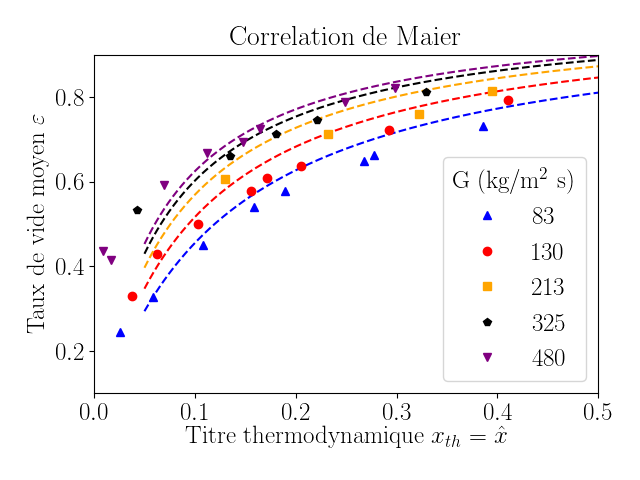
\includegraphics[width=0.47\linewidth]{images/MaierCorrelation.png}
    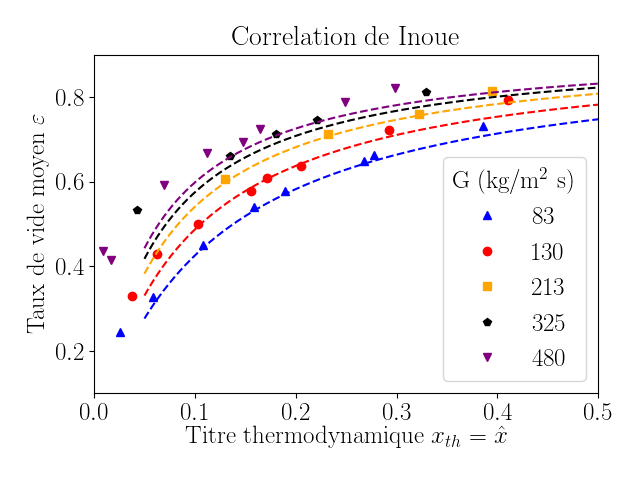
\includegraphics[width=0.47\linewidth]{images/InoueCorrelation.png}
    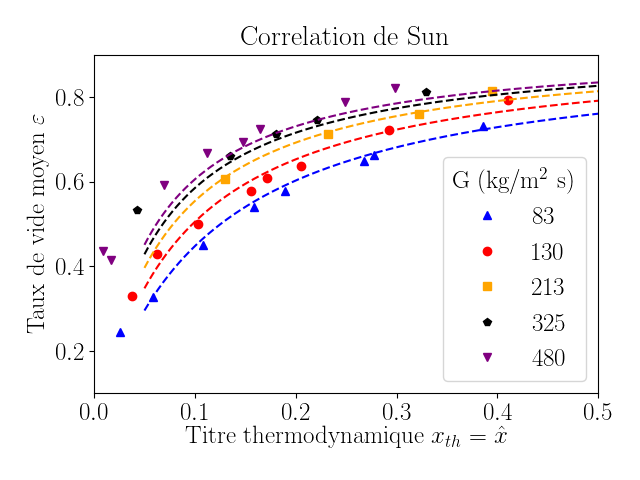
\includegraphics[width=0.47\linewidth]{images/SunCorrelation.png}
    \caption{Comparaison des corrélations de (Maier \& Coddigton, 1997), (Inoue \& al, 1993) et (Sun \& al, 1980) avec les données expérimentales de (Zuber \& al, 1967)}
    \label{fig:Pb3CompExperiment}
\end{figure}